\section{Three-Dimensional Systems and Chaos}
\noindent\rule[\linienAbstand]{\linewidth}{\linienDickeDick}
Chaos is aperiodic long-term behaviour in a deterministic system with sensitive dependence on the initial conditions.\\

Dimension $n \geq 3$: Trajectories can remain bounded without
converging to a fixed point or a closed orbit. Possibly sensitive dependence on the initial conditions, i.e. slightly differing initial conditions lead to a totally different
long-term behaviour

\subsection{Rössler System}
\noindent\rule[\linienAbstand]{\linewidth}{\linienDicke}
The following nonlinear system was constructed by R¨ossler in 1976:
\begin{equation}
  \begin{split}
    \dot{x} &= -(x+z)\\
    \dot{y} &= x + ay\\
    \dot{z} &= b + z(x-c)
  \end{split}
\end{equation}
It depends on the 3 parameters $a, b, c;$ we set $a = 0.2, b = 0.2$ and consider the system for varying values of $c$. Depending on the parameter values, the system has at most two fixed points. Depending on the parameter values, the system has at most two fixed points, namely
\begin{equation}
  \tiny
  P_{1,2} = \left(
  \frac{1}{2} \left( c\mp \sqrt{c^2 - 4ab}\right),
  \frac{1}{2a}\left(-c\pm \sqrt{c^2 - 4ab}\right),
  \frac{1}{2a}\left( c\mp \sqrt{c^2 - 4ab}\right)
  \right)
\end{equation}
The stability of these fixed points can be determined by considering the eigenvalues of the Jacobian of the system. Empirical investigations show that for most parameter values for which the fixed points $P_{1,2}$ exist, at least one of the eigenvalues of the Jacobian matrix has a positive real part and is therefore unstable.\\
% \begin{equation}
%   J = \begin{pmatrix}
%     0 & -1 & -1 \\
%     1 & a & 0 \\
%     z & 0 & x-c
% \end{pmatrix}
% \end{equation}
The behaviour of the Rössler system can vary greatly, depending on the values of the
parameters. For $c = 2.3$ and $c = 2.9$, the system converges to a period-one and a periodtwo limit cycle, respectively. For $c = 8.5$, we observe a chaotic attractor.

\begin{figure}[H]
  \centering
  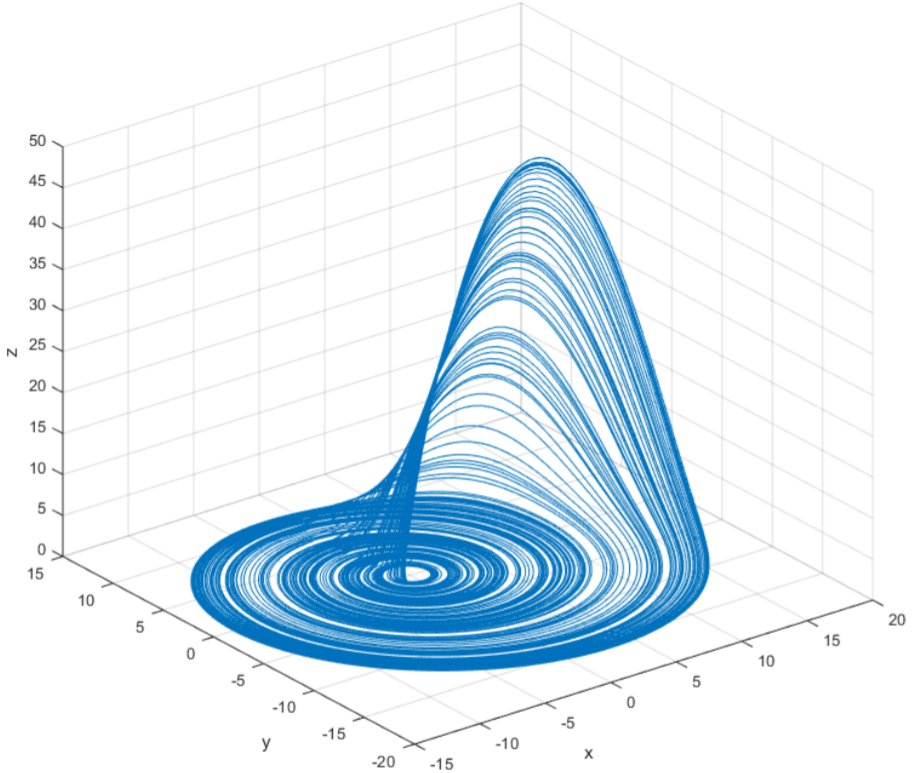
\includegraphics[width=.7\linewidth]{Pics/4.47.png}
\end{figure}

\subsection{Lorenz System}
\noindent\rule[\linienAbstand]{\linewidth}{\linienDicke}
\begin{equation}
  \begin{split}
    \dot{x} &= \sigma(y-x)\\
    \dot{y} &= rx - y - xz\\
    \dot{z} &=-bz + xy
  \end{split}
\end{equation}
We investigate the Lorenz system for the parameter values $\sigma = 10, b = \frac{8}{3}$, and various values of $r$, in most cases $r = 28$.\\
We first determine fixed points of the system. To this end, we solve the system of equations and obtain the three fixed points
\begin{equation}
  P_1^* = (0, 0, 0),\;\;\; P_{2,3}^* = \left(\pm \sqrt{b(r-1)}, \pm \sqrt{b(r-1)}, r-1\right)
\end{equation}
The fixed points $P_2^*$ and $P_3^*$ only exist in the case $r \geq 1$; at the parameter value $r = 1$ there is a bifurcation. The Jacobian of the Lorenz system is
\begin{equation}
  J(x, y, z) =
  \begin{pmatrix}
    \sigma & -\sigma & 0 \\
    r-z & -1 & -x \\
    y & x & -b
  \end{pmatrix}
\end{equation}
At $P_1^*$ the eigenvalues of $J$ are, depending on $r$, with $\sigma = 10$ and $b = \frac{8}{3}$,
\begin{equation}
  \lambda_1 = -\frac{8}{3}, \;\;\; \lambda_{2,3} \frac{1}{2}\left(-11 \pm \sqrt{81 + 40r}\right)
\end{equation}

For $r < 1$ all three eigenvalues are negative and $P_1^*$ therefore a stable fixed point; for $r > 1$, we have $\lambda_2 > 0$, and $P_1^*$ is therefore unstable. Concerning $P_2^*$ and $P_3^*$ , from a corresponding analysis of the eigenvalues we see that these points are stable for $0 < r < r_1 \approx 24.737$ and unstable for $r > r_1$.\\

The greatest degree of instability thus exists in the case $r > r_1$, e.g. for the typical value $r = 28$.

\begin{figure}[H]
  \centering
  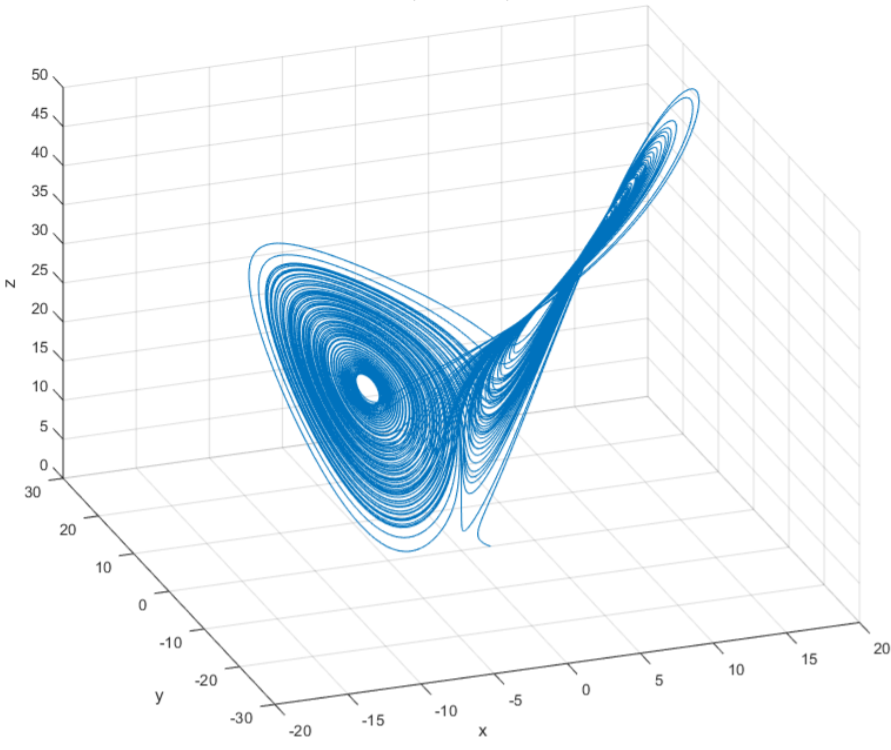
\includegraphics[width=.7\linewidth]{Pics/4.54.png}
\end{figure}

\subsection{Linz/Sprott System}
\noindent\rule[\linienAbstand]{\linewidth}{\linienDicke}
One of the simplest examples of a 3-dimensional continuous system exhibiting chaotic dynamics is the following nonlinear third-order ODE.
\begin{equation}
  x^{(3)} + a \ddot{x} + b\dot{x} - |x| + 1 = 0
\end{equation}
Note that the absolute value $|x|$ is the only nonlinearity on the system.\\
A simulation of the system for $a = 0.6, b = 1$ (and the initial conditions $x(0) = -0.1, y(0) = z(0) = 0$) shows that the system converges to a chaotic attrator which somewhat resembles a Möbius strip:

\begin{figure}[H]
  \centering
  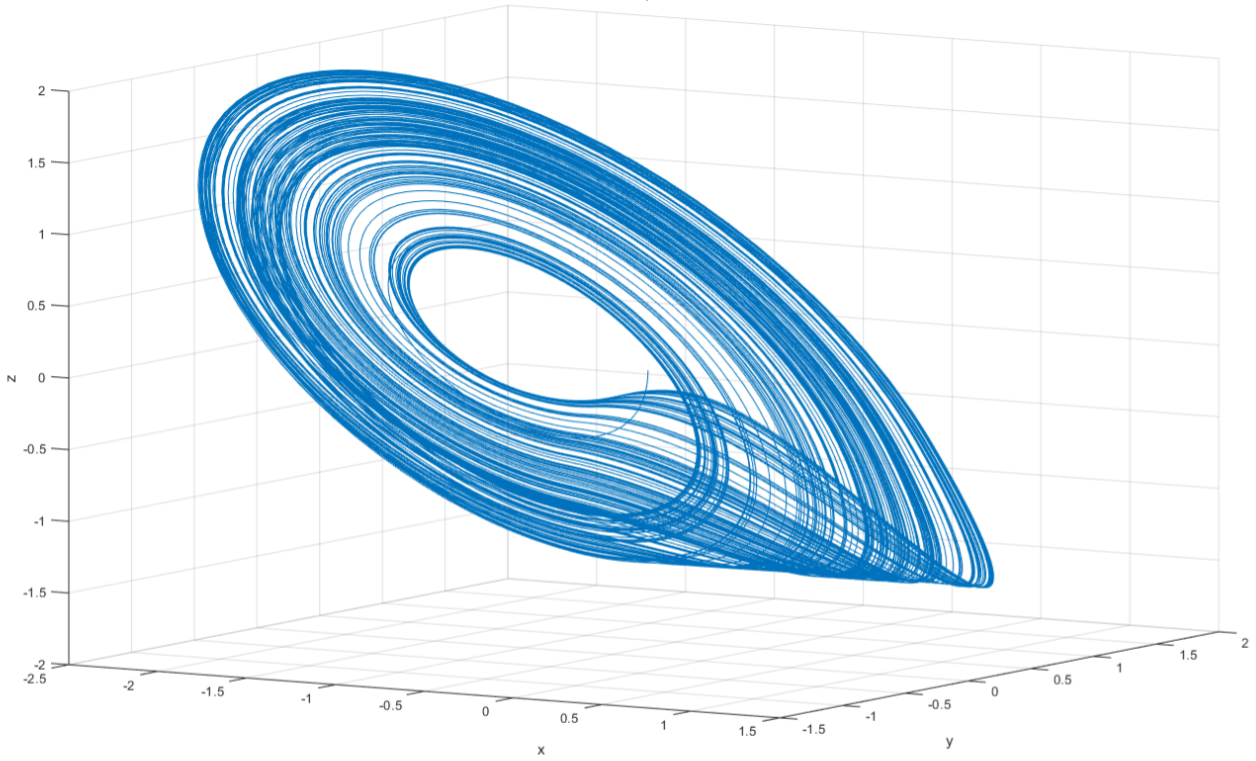
\includegraphics[width=.7\linewidth]{Pics/4.58.png}
\end{figure}
\vfill\null
\columnbreak
